\documentclass[pdflatex,sn-mathphys-num]{sn-jnl}

\usepackage{graphicx}
\usepackage{listings}
\usepackage{xcolor}
\usepackage{booktabs}
\usepackage{float}
\usepackage{caption}
\usepackage{subcaption}
\usepackage{amsmath}
\usepackage{tcolorbox}
\usepackage{lipsum}
\usepackage{multirow}
\usepackage{mathrsfs}
\usepackage{amssymb}
\usepackage{algorithm}
\usepackage{algpseudocode}

\begin{document}

\title{New Generation Data Models and Dbmss Course - Assignment 2 - Crowdfunding Company}

\author*[1]{\fnm{Carlo} \sur{Falchi (Matr. 67340A)}}\email{carlo.falchi@studenti.unimi.it}
\author*[1]{\fnm{Francesco} \sur{Palladini (Matr. 85652A)}}\email{francesco.palladini@studenti.unimi.it}
\affil[1]{\orgdiv{Department of Computer Science}, \orgname{University of Milan}, \country{Italy}}

\maketitle
\begin{figure}[ht]
    \centering
    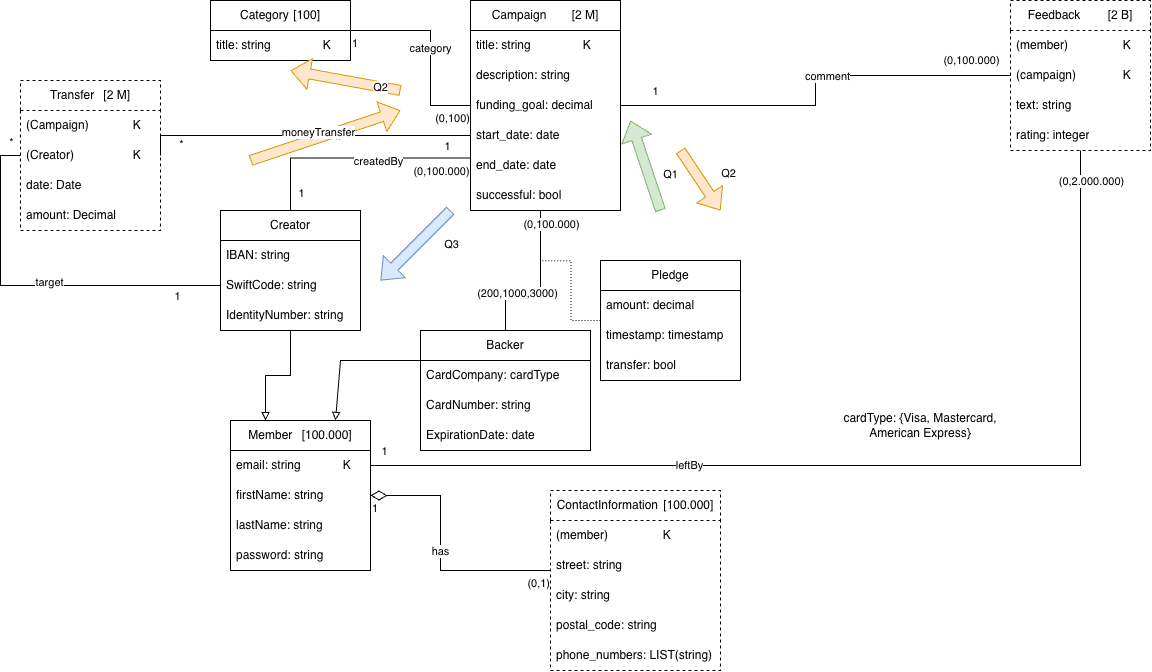
\includegraphics[width=0.9\textwidth]{figures/workloadv6.png}
    \caption{UML Diagram}
     \label{fig:uml}
\end{figure}
\section{Solution}

\subsection{Logical Model}
\begin{figure}[ht]
    \centering
    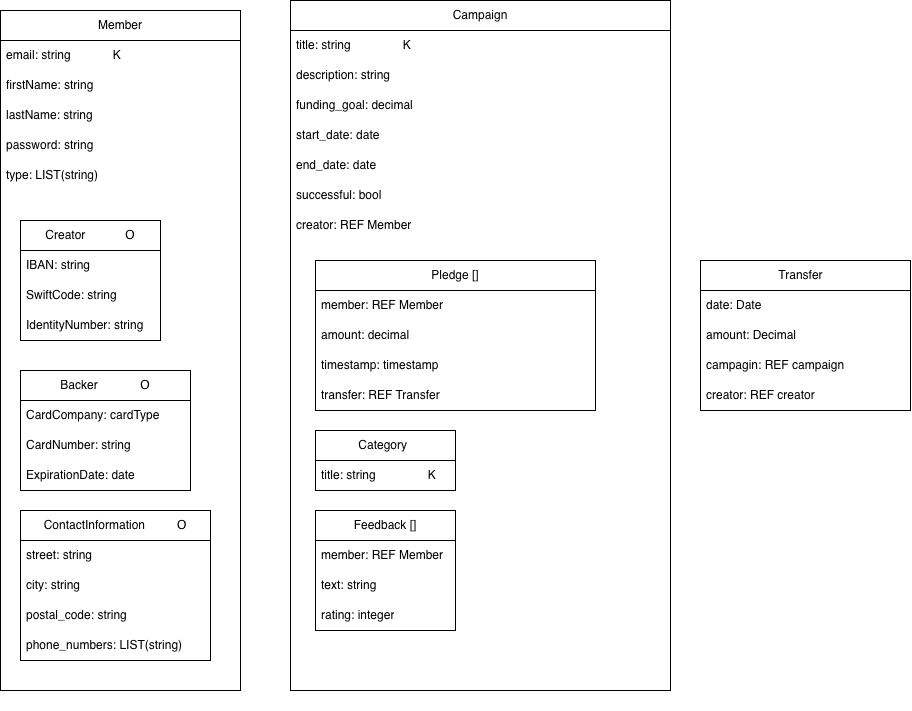
\includegraphics[width=0.9\textwidth]{figures/logicalmodel.png}
    \caption{Logical Model}
     \label{fig:logical}
\end{figure}
Workload to consider:
\begin{enumerate}
    \item Identify the top 5 most competitive campaigns, i.e., those that received the highest
number of pledges.
    \item For each campaign creator, identify the category in which they achieved the highest
average pledge amount.
    \item For each month in the last year, identify the top 10 creators per month, i.e., the creators
who completed the highest number of successful campaigns in that month
\end{enumerate}

The figure \ref{fig:uml} shows the navigational path for the three worloads:
\begin{itemize}
    \item Q1:(Pledge)$\to$(Campaign)
    \item Q2:((Creator)$\underset{creator}{\to}$(Campaign)$\to$(Pledge) and Campaign$\underset{category}{\to}$Category to identify the titles of categories
    \item Q3:((Campaign)$\underset{createdBy}{\to}$(Creator)
\end{itemize}

The figure \ref{fig:logical} reports the logical model that we have realized taking into account the above operations.
The first operation uses Pledge as an entry point, the second uses Creator and the third uses Campaign,
Q1 and Q2 are in conflict because they have different directions, however the Campaign is used in all the workloads.
Furthermore, given that a Pledge can be assigned to only one Campaign we suggest using Campaign as an entry point and thus  as a collection and embedding 
pledge in it without risk of duplication.
To improve the performance of the second operation (Campaign $\to$ Category) we embedded category inside the Campaign
so we can avoid the lookup operation, it can introduce duplication but it is considered acceptable.
Regarding the third operation (Campaign $\to$ Creator), which uses Campaign as entry point, it confirms
the need to use campaign as a collection and Creator as a reference using a lookup to avoid duplication of Creators.
The feedback collection has been embedded within campaign, given that there is a one-to-many relationship 
between campaign and feedback, and to avoid duplication we use a reference to the Member class. 
The Transfer collection has been created as a separate collection because it is
not included in the most important workloads, we expect that a report or a page will request all transfers
rarely so we can insert Campaign and Creator as a reference and use the lookup operation for them.
Finally the Member collection has been created as an entry point and as a separate collection, embedding in it 
its specializations Creator and Member. Optional contact information has been embedded in it but there are further
improvements explained in the next section.

My suggestion:

Embedding Transfer into Campaign, because the asociation between Transfer and Campaign is one to many, and Transfer is in
the side many. An other reason is to make the computed pattern more efficient, because otherwise I would have to make the
lookup every time the amount in Transfer is updated.

\subsection{Design Patterns}
My suggestions:
computedpattern: totaleAmount, numberPledges
reference pattern: creatoreName in Campaign, backerName in Pledge
sub pattern: ContactInformation separated
version pattern: to keep version info

First, in order to save computations, we can apply the computed pattern to the attribute amount in Transfer. We can use the extended reference pattern by 
dupicating the attributes firstName and lastName of Creator in the Campaign class, to make faster the execution of query 2 and 3. 
We can also apply the subset pattern by creating a separate collection for ContactInformation, which is not involved in the workload, 
and so we expect that it is accessed less often.

\end{document}